\documentclass{article}
\usepackage[landscape,letterpaper,left=1cm,right=1cm,top=1cm,bottom=1cm]{geometry}

\usepackage{booktabs}
\usepackage[type={CC},modifier={by-sa},version={4.0}]{doclicense}
\usepackage[inline,shortlabels]{enumitem}
\usepackage{graphicx}
\usepackage[colorlinks,urlcolor=blue]{hyperref}
\usepackage{multicol}
\usepackage{parskip}            % stop indenting

\usepackage{color}
\definecolor{macewan}{RGB}{151,29,56}

\usepackage[compact]{titlesec}
\titleformat{\section}{\normalfont\color{macewan}\fontsize{11}{12}\bfseries}{\thesection}{0ex}{}
\titlespacing{\section}{0pt}{0.2\baselineskip}{0.1\baselineskip}
\titleformat{\subsection}{\normalfont\fontsize{8}{9}\bfseries}{\thesection}{0ex}{}
\titlespacing{\subsection}{0pt}{0.2\baselineskip}{0.1\baselineskip}

\usepackage{fancyhdr}
\pagestyle{empty}

\usepackage{xltxtra}
\setmainfont[Ligatures=TeX]{Helvetica Neue}
\setmonofont[AutoFakeSlant,BoldItalicFeatures={FakeSlant}]{Courier}

\usepackage{listings}
\usepackage{listings-golang}
\lstdefinelanguage{plain}{%
  basicstyle=\ttfamily,
  keywordstyle={},
  identifierstyle={},
  commentstyle={},
  stringstyle={},
}
\definecolor{identifiers}{RGB}{90,0,0}
\definecolor{comments}{RGB}{0,90,0}
\definecolor{keywords}{RGB}{0,0,130}
\lstset{language=Golang,
  morekeywords={go},
  escapechar=_,
  basicstyle=\footnotesize\ttfamily,
  commentstyle=\color{comments}\emph,
  identifierstyle=\color{identifiers},
  keywordstyle=\color{keywords}\bfseries,
  breaklines=true,
  frame=none,
  numbers=none,
  numbersep=5pt,
  numberstyle=\footnotesize,
  stepnumber=1,
  stringstyle=\ttfamily,
  belowskip=0.2\baselineskip,
  aboveskip=0.2\baselineskip,
}

\newcommand{\var}[1]{\texttt{\textit{\underbar{#1}}}}

\begin{document}

\raggedright

\begin{multicols*}{3}
  \footnotesize

  \begin{center}
    {\Large{}\bfseries{}Go Reference Card}

    Dr. Nicholas M. Boers\\
    \url{boersn@macewan.ca}\\
    \IfFileExists{macewan.pdf}{
      \vspace{0.2em}
      
\includegraphics[height=0.85cm]{macewan}
    }{
      MacEwan University
    }

    \vspace{1em}
    Last updated: \today
  \end{center}

  \filbreak
  \section*{Introduction}

  \subsection*{Synopsis}

\begin{lstlisting}[language=plain,escapechar=|]
go |\var{command}| [|\var{arguments}|]
\end{lstlisting}

  Commands:

  \begin{tabular}{p{0.5in}p{2.5in}}
    \texttt{build} & compile packages and dependencies \\
    \texttt{get} & download and install packages and dependencies \\
    \texttt{run} & compile and run Go program \\
  \end{tabular}

  \subsection*{Program execution}

  Execution begins at the function \lstinline{main} in package \lstinline{main}:
\begin{lstlisting}[frame=single,escapechar=\%]
package main

func main() {
    // body for function
}
\end{lstlisting}

  \filbreak
  \section*{Variables}

  \begin{tabular}{p{0.5in}p{2.5in}}
    \toprule
    \textbf{Type} & \textbf{Description} \\
    \midrule
    \texttt{string} & sequence of immutable bytes\newline{}
                      \texttt{"\dots"}: interpreted string literal\newline{}
                      \texttt{`\dots`}: raw string literal (no backslash escapes)\\
    \texttt{bool} & Boolean value; either \texttt{true} or \texttt{false} \\
    \texttt{int} & signed 32- or 64-bit integer \\
    \texttt{uint} & unsigned 32- or 64-bit integer \\
    \texttt{int\textit{\underbar{x}}} & signed \texttt{\textit{\underbar{x}}}-bit integer where \texttt{\textit{\underbar{x}}} is 8, 16, 32, or 64 \\
    \texttt{uint\textit{\underbar{x}}} & unsigned \texttt{\textit{\underbar{x}}}-bit integer \\
    \texttt{float\textit{\underbar{x}}} & \texttt{\textit{\underbar{x}}}-bit float where \texttt{\textit{\underbar{x}}} is 32 or 64 \\
    \bottomrule
  \end{tabular}

  \filbreak
  \subsection*{Declarations}

  \begin{tabular}{p{1.25in}p{1.75in}}
    \toprule
    \textbf{Syntax} & \textbf{Description} \\
    \midrule
    \lstinline!var id T! & declare \lstinline!id! as type \lstinline!T! and init to \lstinline!T!'s zero value\\
    \lstinline!var id T = val! & declare \lstinline!id! as type \lstinline!T! and init to \lstinline!val! \\
    \lstinline!var id = val! & declare \lstinline!id! and init to \lstinline!val! \\
    \lstinline!id := val! & declare \lstinline!id! and init to \lstinline!val! \\
    \bottomrule
  \end{tabular}

  \filbreak
  \subsection*{Miscellaneous}

  \begin{tabular}{p{1.25in}p{1.75in}}
    \toprule
    \textbf{Syntax} & \textbf{Description} \\
    \midrule
    \lstinline!T(val)! & convert \lstinline!val! to type \lstinline!T! \\
    \lstinline!compType{elem, !\texttt{\dots}\lstinline!}! & create composite literal where \lstinline!compType! is a struct, array, slice, map, \dots{} consisting of \lstinline!elem!, \texttt{\dots} \\
    \bottomrule
  \end{tabular}


  \filbreak
  \section*{Keywords, operators, delimiters}

  \begin{tabular}{p{0.44in}p{0.74in}p{0.35in}p{0.6in}p{0.7in}}
    \lstinline!break!    & \lstinline!default!     & \lstinline!func!   & \lstinline!interface! & \lstinline!select!\\%
    \lstinline!case!     & \lstinline!defer!       & \lstinline!go!     & \lstinline!map!       & \lstinline!struct!\\%
    \lstinline!chan!     & \lstinline!else!        & \lstinline!goto!   & \lstinline!package!   & \lstinline!switch!\\%
    \lstinline!const!    & \lstinline!fallthrough! & \lstinline!if!     & \lstinline!range!     & \lstinline!type!\\%
    \lstinline!continue! & \lstinline!for!         & \lstinline!import! & \lstinline!return!    & \lstinline!var!\\%
  \end{tabular}

  Operators, delimiters, and other special tokens:

  \begin{tabular}{lllllllll}
    \verb!+! & \verb!& ! & \verb!+=! & \verb!&= ! & \verb!&&! & \verb+==+ & \verb+!= + & \verb!(! & \verb!)! \\
    \verb!-! & \verb!| ! & \verb!-=! & \verb!|= ! & \verb!||! & \verb+< + & \verb+<= + & \verb![! & \verb!]! \\
    \verb!*! & \verb!^ ! & \verb!*=! & \verb!^= ! & \verb!<-! & \verb+> + & \verb+>= + & \verb!{! & \verb!}! \\
    \verb!/! & \verb!<<! & \verb!/=! & \verb!<<=! & \verb!++! & \verb+= + & \verb+:= + & \verb!,! & \verb!;! \\
    \verb!%! & \verb!>>! & \verb!%=! & \verb!>>=! & \verb!--! & \verb+! + & \verb+...+ & \verb!.! & \verb!:! \\
    \verb! ! & \verb!&^! & \verb!  ! & \verb!&^=! & \verb!  ! & \verb+  + & \verb+   + & \verb! ! & \verb! ! \\
  \end{tabular}

  Notable differences from C:

  \begin{tabular}{ll}
    \texttt{\&\textasciicircum} & bit clear (AND NOT) \\
    \texttt{\&\textasciicircum=} & bit clear (AND NOT) to update a variable \\
    \texttt{<-} & channel send/receive \\
    \texttt{:=} & short variable declaration     \\
  \end{tabular}

  \filbreak
  \section*{Functions}

  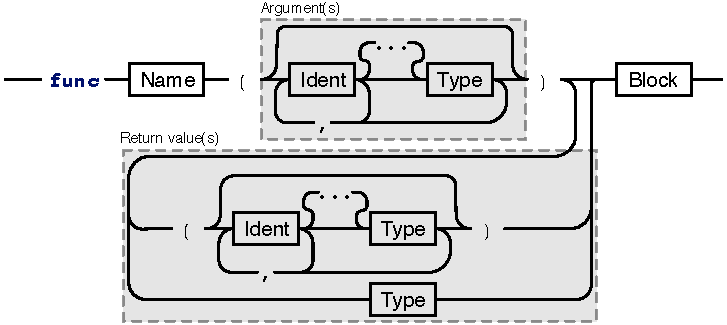
\includegraphics[width=\linewidth]{func}

  \begin{tabular}{p{0.3in}p{2.7in}}
    Block & statement list inside braces, similar to C\newline(e.g.,~\lstinline!{ failures++; }!)\\
  \end{tabular}

  \vspace{\baselineskip}
\begin{lstlisting}[frame=single]
func double(val *int) {
    val *= 2
}

func pedanticRoot(a float64) (float64, float64) {
    root := math.Sqrt(a)
    return root, -root
}
\end{lstlisting}

  \filbreak
  \section*{Control structures}

  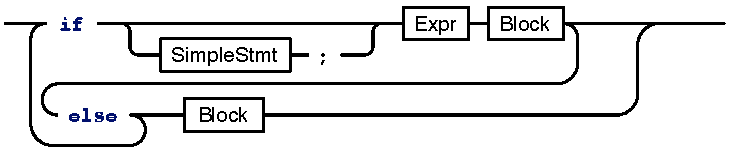
\includegraphics[width=\linewidth]{if}

  \begin{tabular}{p{0.6in}p{2.4in}}
    SimpleStmt & expression, increment/decrement statement (e.g.,~\lstinline!i++!), assignment (e.g.,~\lstinline!count = 0!), short declaration (e.g.,~\lstinline!count := 0!)\\
    Expr & expression, similar to C (e.g.,~\lstinline!count > 10!)\\
  \end{tabular}

  \vspace{\baselineskip}
\begin{lstlisting}[frame=single,escapechar=|]
if bal < 0 {
    // body for bal < 0
} else if bal < 10000 {
    // body for bal < 10000
} else {
    // body for bal >= 10000
}

if err := f.Close(); err != nil {
    // body
}
\end{lstlisting}

  \filbreak
  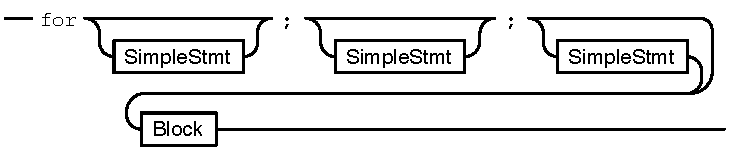
\includegraphics[width=\linewidth]{for-3parts}

\begin{lstlisting}[frame=single,escapechar=|]
for i := 0; i < 10; i++ {
    // body for C-style "for" loop
}
for ;; {
    // body for C-style |\color{comments}$\infty$| "for" loop
}
\end{lstlisting}

  \filbreak
  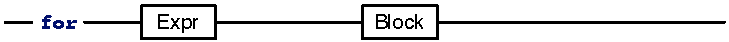
\includegraphics[width=\linewidth]{for-1cond}

  \begin{minipage}{0.47\linewidth}
\begin{lstlisting}[frame=single,escapechar=|]
for count < 100 {
    // "while" loop
}
\end{lstlisting}
  \end{minipage}\hfill%
  \begin{minipage}{0.47\linewidth}
\begin{lstlisting}[frame=single,escapechar=|]
for {
    // |\color{comments}$\infty$| "while" loop
}
\end{lstlisting}
  \end{minipage}

  \filbreak
  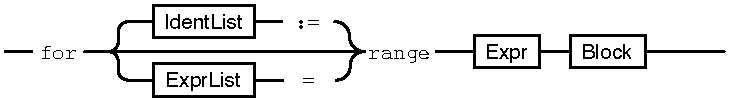
\includegraphics[width=\linewidth]{for-range}

  \begin{tabular}{p{0.35in}p{2.65in}}
  IdentList & identifiers separated by commas (e.g.,~\lstinline!i, j, k!) \\
  ExprList & expressions separated by commas (e.g.,~\lstinline!key, val!) \\
  \end{tabular}

  \vspace{\baselineskip}
\begin{lstlisting}[frame=single,escapechar=|]
for idx, str := range []string{"A", "B", "C"} {
    // body for Python-style "for" loop
    fmt.Println(idx, str)
}
\end{lstlisting}

  \filbreak
  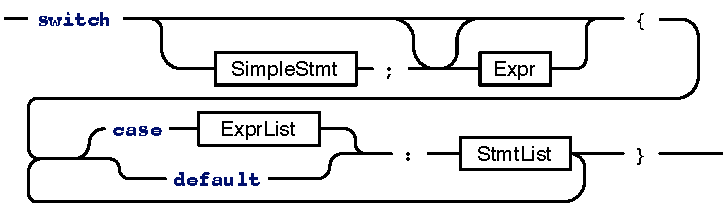
\includegraphics[width=\linewidth]{switch-expr}

  Note that a \lstinline{switch} may have at most one \lstinline{default} case.

  \filbreak
  \section*{Standard library}

  \begin{tabular}{p{0.8in}p{2.2in}}
    \toprule
    \textbf{Package} & \textbf{Description} \\
    \midrule
    \texttt{database/sql} & generic interface around SQL DBs \\
    \texttt{encoding/csv} & read/write CSV files \\
    \texttt{encoding/json} & encode/decode JSON \\
    \texttt{errors} & manipulation of errors \\
    \texttt{flag} & command-line argument parsing \\
    \textbf{\texttt{fmt}} & formatted I/O, e.g., \texttt{Printf} \\
    \texttt{log} & simple logging\\
    \texttt{math/rand} & pseudo-random number generators \\
    \textbf{\texttt{net/http}} & HTTP client/server implementations \\
    \texttt{os} & interface to OS functionality \\
    \texttt{path} & manipulation of slash-separated paths \\
    \texttt{sort} & primitives for sorting \\
    \textbf{\texttt{strings}} & string manipulation (UTF-8 encoded) \\
    \texttt{time} & functionality for measuring/displaying time \\
    \bottomrule
  \end{tabular}

  \filbreak
  \section*{Pointers}

  \begin{tabular}{p{0.48in}p{2.52in}}
    \toprule
    \textbf{Syntax} & \textbf{Description} \\
    \midrule
    \lstinline!*int! & type: pointer to an \texttt{int} \\
    \lstinline!*[]int! & type: pointer to a slice of \texttt{int} \\
    \lstinline!*[4]int! & type: pointer to an array of 4 \texttt{int} \\
    \midrule
    \texttt{\&x} & if \texttt{x} is of type \texttt{T}, pointer to \texttt{x} (of type \texttt{*T}) \\
    \texttt{*x} & if \texttt{x} is of type \texttt{*T}, variable pointed to by \texttt{x} (of type \texttt{T}) \\
    \bottomrule
  \end{tabular}

  \filbreak
  \section*{map}

  \begin{tabular}{p{1.5in}p{1.5in}}
    \toprule
    \textbf{Syntax} & \textbf{Description} \\
    \midrule
    \lstinline!map[string]int! & type: map string $\rightarrow$ int \\
    \lstinline!map[int]float64! & type: map int $\rightarrow$ float64 \\
    \midrule
    \lstinline!m := make(map[int]int)! & create a new/empty map \\
    \lstinline!m := map[int]int{}! & create a new/empty map \\
    \lstinline!m[1337] = 42! & set a key/value pair \\
    \lstinline!m[1337]! & access a key/value pair \\
    \bottomrule
  \end{tabular}

  \filbreak
  \section*{slices}

  \begin{tabular}{p{0.75in}p{2.25in}}
    \toprule
    \textbf{Syntax} & \textbf{Description} \\
    \midrule
    \texttt{[]\var{T}} & type: slice of type \var{T} \\
    \midrule
    \texttt{\var{var}[\var{low}:\var{high}]} & slice of \var{var} from \var{low} to \var{high} (not incl. \var{high}) \\
    \texttt{\var{var}[\var{low}:]} & slice of \var{var} from \var{low} to \texttt{len(\var{var})} \\
    \texttt{\var{var}[:\var{high}]} & slice of \var{var} from 0 to \var{high} (not incl. \var{high})\\
    \texttt{\var{var}[:]} & slice of \var{var} from 0 to \texttt{len(\var{var})} \\
    \bottomrule
  \end{tabular}

  \filbreak
  \section*{struct}

  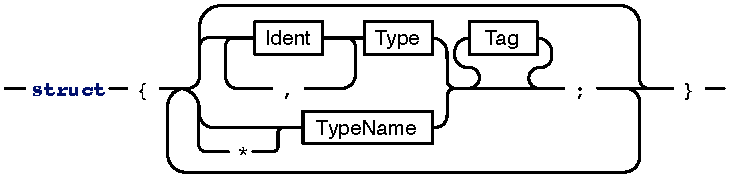
\includegraphics[width=\linewidth]{struct}

  \begin{tabular}{p{0.45in}p{2.55in}}
  Ident &  identifier \\
  Type &  an array, struct, pointer, function, interface, slice, map, or channel type; or a TypeName \\
  TypeName &  identifier for a user-defined type \\
  Tag &  an optional string literal used to specify an attribute for a field \\
  \end{tabular}

  \vspace{\baselineskip}

\begin{lstlisting}[frame=single]
struct {
    T           // embedded field, e.g., a
    x, y int    // struct of type T
    u float32   `json:"u"` // example tag
    A *[]int
    F func()
}
\end{lstlisting}

  \filbreak
  \section*{User-defined types}

  \begin{tabular}{p{0.75in}p{2.25in}}
    \toprule
    \textbf{Syntax} & \textbf{Description} \\
    \midrule
    \lstinline!type!\texttt{ \var{id} \var{T}} & define new type \var{id} with underlying type \var{T} \\
    \midrule
    \begin{minipage}{0.7in}
\begin{lstlisting}[escapechar=|]
type (
    |\var{id} \var{T}|
    |\var{id} \var{T}|
    |\dots|
)
\end{lstlisting}
    \end{minipage}
                    & define several new types at once\\
    \bottomrule
  \end{tabular}

  \vspace{\baselineskip}
\begin{lstlisting}[frame=single]
type Point struct {
    x, y int
}

type TreeNode struct {
    left, right *TreeNode
    value *Comparable
}
\end{lstlisting}

  \filbreak
  \section*{Methods}

  The syntax is identical to {\color{macewan}\bfseries{}Functions} except for the addition of \texttt{(\var{rcvr})}, which is essentially an identifier and type.

\begin{lstlisting}[escapechar=|]
func (|\var{rcvr}|) |\var{name}|(|\var{args}|) |\var{return}| {
    // function body
}
\end{lstlisting}

\begin{lstlisting}[frame=single,escapechar=|]
func (p *Point) Scale(factor float64) {
    p.x *= factor
    p.y *= factor
}

func (p *Point) Length() float64 {
    return math.Sqrt(p.x * p.x + p.y * p.y)
}
\end{lstlisting}

  \filbreak
  \section*{Interfaces}

  An interface type describes \textit{behaviour}, rather than data.
  An object's type is equivalent to the interface type if the object implements the interface type's behaviour.

\begin{lstlisting}[escapechar=|]
type |\var{name}| interface {
    // "name(arguments) return", one per line
}
\end{lstlisting}

\begin{lstlisting}[escapechar=|]
type ReadCloser interface {
    Reader
    Closer
}
type Reader interface {
    Read(p []byte) (n int, err error)
}
type Closer interface {
    Close() error
}
\end{lstlisting}

  \filbreak
  \section*{Error}

The predeclared type error is defined as

\begin{lstlisting}
type error interface {
    Error() string
}
\end{lstlisting}

  \parbox{\columnwidth}{
    \section*{References}

    \begin{itemize}[nosep]
    \item \texttt{go --help}
    \item \url{https://golang.org/ref/spec}
    \item \url{https://github.com/a8m/go-lang-cheat-sheet}
    \item \url{http://www.math.brown.edu/~jhs/ReferenceCards/CRefCard.v2.2.pdf}
    \end{itemize}

    \vspace{\baselineskip}
    \begin{center}
      \doclicenseText\\[0.25\baselineskip]

      \doclicenseImage
    \end{center}
  }
\end{multicols*}

\end{document}
